\documentclass[]{auvsi_doc}
\setkeys{auvsi_doc.cls}{
	AUVSITitle={Concept Selection Matrix},
	AUVSILogoPath={./figs/logo.pdf}
}

% include extra packages, if needed
\usepackage{multirow}
\usepackage{rotating}
\usepackage{tabularx}

\begin{document}

\begin{AUVSITitlePage}
\begin{artifacttable}
\entry{AF-003, 1.0, 10-31-2018, Concept development initial stage, Ryan Anderson, Andrew Torgesen}
\entry{AF-003, 1.1, 11-06-2018, Concept development first revision, Ryan Anderson, }
% additional \entry{} commands for extra rows in the revision table, if needed
\end{artifacttable}
\end{AUVSITitlePage}

% document contents (see below for LaTex commands that make your life easier)

\newpage
\begin{sidewaystable}
\begin{center}
	\captionof{table}{Concept Selection Matrix for the airframe. Metrics for each concept are multiplied by their respective \textbf{Metric Weight} and summed to provide an overall comparison rating.} \label{tab:proj_app}
	\begin{tabular}{|p{2.5cm}|p{1.5cm}|p{1.5cm}|p{1.5cm}|p{1.5cm}|p{2cm}|p{2cm}|p{2cm}|p{1.5cm}|p{1.5cm}|}
		\hline	
		\rowcolor[HTML]{C0C0C0}	
		{\color[HTML]{000000} \textbf{Metric}} & {\color[HTML]{000000} \textbf{Metric Weight}} & {\color[HTML]{000000} \textbf{My Twin Dream}} & {\color[HTML]{000000} \textbf{Nimbus Pro}} & {\color[HTML]{000000} \textbf{Titan}} & {\color[HTML]{000000} \textbf{Modified My Twin Dream}} & {\color[HTML]{000000} \textbf{Modified Nimbus Pro}} & {\color[HTML]{000000} \textbf{Custom Traditional Fixed Wing}} & {\color[HTML]{000000} \textbf{Custom Flying Wing}} & {\color[HTML]{000000} \textbf{Hexa copter}} \cr \hline
		
		\centering{\textbf{Wing Area}} & \centering{\textbf{2}} & \centering{3} & \centering{4} & \centering{4} & \centering{5} & \centering{5} & \centering{5} & \centering{5} & \centering{5} \cr \hline
		
		\centering{\textbf{Weight}} & \centering{\textbf{2}} & \centering{3} & \centering{2} & \centering{2} & \centering{3} & \centering{2} & \centering{4} & \centering{5} & \centering{4} \cr \hline
		
		\centering{\textbf{Wing Loading}} & \centering{\textbf{4}} & \centering{3} & \centering{4} & \centering{4} & \centering{5} & \centering{5} & \centering{5} & \centering{5} & \centering{5} \cr \hline 
		
		\centering{\textbf{Volume Capacity}} & \centering{\textbf{4}} & \centering{3} & \centering{4} & \centering{5} & \centering{3} & \centering{4} & \centering{4} & \centering{1} & \centering{5} \cr \hline
		
		\centering{\textbf{Stability Control}} & \centering{\textbf{2}} & \centering{3} & \centering{3} & \centering{2} & \centering{3} & \centering{4} & \centering{4} & \centering{2} & \centering{5} \cr \hline
		
		\centering{\textbf{Build Time}} & \centering{\textbf{5}} & \centering{3} & \centering{3} & \centering{3} & \centering{2} & \centering{2} & \centering{1} & \centering{2} & \centering{2} \cr \hline
		
		\centering{\textbf{Monetary Cost}} & \centering{\textbf{1}} & \centering{3} & \centering{3} & \centering{3} & \centering{2} & \centering{2} & \centering{4} & \centering{4} & \centering{1} \cr \hline
		
		\centering{\textbf{Range}} & \centering{\textbf{5}} & \centering{3} & \centering{3} & \centering{3} & \centering{3} & \centering{3} & \centering{3} & \centering{3} & \centering{1} \cr \hline

		\centering{\textbf{Controls Implementation}} & \centering{\textbf{5}} & \centering{3} & \centering{3} & \centering{2} & \centering{3} & \centering{3} & \centering{2} & \centering{1} & \centering{1} \cr \hline

		\centering{\textbf{Totals}} & \centering{\textbf{-}} & \centering{\textbf{90}} & \centering{\textbf{98}} & \centering{\textbf{95}} & \centering{\textbf{96}} & \centering{\textbf{100}} & \centering{\textbf{96}} & \centering{\textbf{82}} & \centering{\textbf{85}} \cr \hline

	\end{tabular}
	
	% \end{table}
\end{center}
\end{sidewaystable}

\section{Concept Selection Metrics}

In general, metrics used in concept selection of the airframe were inspired by the Airframe System Requirements Matrix. These were in turn inspired by the generalized System Requirements and our Key Success Measures. Based on these documents, it was determined that one of the most important requirements for the concept are its build time. This is in light of a crash shortly before last year's competition that required a radical design change. Since not enough time was available to rebuild the original design, last year's team purchased an airframe. In order to prevent such an accident from recurring, we hope to optimize build time. As a second consideration, any change in airframe design will require some adjustment to our controls algorithm. Consequently, the estimated time needed for controls adaptation is another metric for our concept selection matrix.\\

Additionally, the two parts of the competition with the most room for improvement over last year's performance are object detection and payload delivery. A slower flight speed with greater stability would allow for sharper image capture as well as a less-complicated payload drop. In order to measure this, it was determined that wing area, airframe weight, wing area-to-weight ratio, and stability would be valuable metrics for selecting a concept that would maximize our performance in these competition tasks.\\

Other more obvious requirements for the airframe include sufficient volume capacity for components and payload, sufficient range to carry out the mission, and low enough cost to remain in budget. These were also included as concept selection metrics.

\section{Metric Scoring}

Concept selection metrics were evaluated by comparing their estimated outcomes to the airframe used in last year's competition. Where possible, quantitative specifications were obtained online for metrics such as wing loading, wing area, weight, cost, and volume capacity. Range was measured primarily to show distinction between fixed wing and copter concepts. Other metrics were evaluated more qualitatively, as in the estimated difficulty for controls implementation and stability.

\section{Concept Selection Idea Descriptions}

\subsection{My Twin Dream (MTD)(\$170)}

Last year's airframe used the MTD design as a last minute replacement for their custom airframe that crashed. As shown in Figure \ref{planes1}, MTD is a twin propulsion fixed wing aircraft. It's made of a sturdy and durable foam (EPO) with a wingspan of 1.8  m, a length of 1.3 m, and weighs about a kilogram (without components). The MTD airframe performed fairly well for last year's team. It had the necessary stability, range, and endurance to complete the competition mission. Some disadvantages are that the plane flew too fast during the competition and didn't have enough room in the fuselage for the water bottle payload. The latter is especially relevant this year because our payload is now a UGV. As an off-the-shelf product, MTD is fairly easy to assemble and rebuild if needed. It's durability also minimizes needed repair upon crashing. MTD is already integrated with ROSPlane and would only need fine tuning of the controls at this point. We used this as the reference design in our concept selection matrix.

\subsection{My Fly Dream Nimbus Pro (\$190)}

Similar to MTD, the Nimbus Pro from My Fly Dream (Figure \ref{planes1}) is also a twin propulsion fixed wing aircraft. Some advantages to this design include a larger wing span (1.95m) and a larger fuselage compartment. The larger wing span can help this plane fly at a slower velocity, although this advantage is offset slightly by a larger weight. The increased fuselage storage room will also give us a better chance of fitting our UGV payload. We estimate Nimbus Pro to be very similar to MTD in other metrics such as stability, time to assemble/rebuild, cost, range, and controls adaptation.

\subsection{Skywalker Titan (\$260)}

The Skywalker Titan is another large fixed-wing airframe we would be able to purchase (Figure \ref{planes1}). Titan has the largest wing span and payload storage capacity of the three off-the-shelf options we are considering. A unique feature to this design is the V-tail in lieu of the traditional tail. This would be difficult and time consuming to adapt for in the controls because now the elevator and rudder control surfaces are combined. Adjusting these combined surfaces would affect the dynamics differently than would the traditional control surfaces. We have also heard through our sponsor, Dr. McLain, that one of his students would not recommend this plane because it is difficult to fly (even without autopilot enabled).

\subsection{Modified My Twin Dream}

One major disadvantage to off-the-shelf products is that they are designed for us; we have no control over optimizing certain design parameters to improve the airframe performance. Another design we considered is taking the same MTD plane we already have and using custom wings that we would design. With this we would be able to improve performance (e.g. increasing wing area to fly slower) without using all our time on designing an entire airframe. Last year's team designed their own airframe, which took a lot of their time and ultimately resulted in a crash. This modified MTD design would maintain the same cost, controls adaptability, durability, and time required to assemble/rebuild as MTD. We would be able to design the wing to fit with the current MTD design and make multiple wings as backup in case of wing failure when crashing or landing. One reason time to rebuild is so vital to this project is that every other subsystem (controls, vision, network, UGV, etc.) is dependent on the airframe working and able to fly. If the plane was damaged and we needed to adjust our design, the other subsystems would not need to wait any longer than they would for normal repairs for MTD. In the meantime, they could fly the plane with the normal MTD wings until we had the new wings designed and made. Another advantage of this idea is that it would give us more learning experience in airframe design than using MTD on its own.

\subsection{Modified Nimbus Pro}

This design is very similar to the Modified MTD (see above). We would have the durability, trusted flight dynamics, and fast time to rebuild as an off-the-shelf plane with the added benefit of the increased wing area (we can only replace part of the wing, so the original wing design is still impactful) and increased storage capacity for the UGV payload. We would also have some control over stability. This combination of benefits is why we have chosen this as our chosen concept.

\subsection{Custom Fixed Wing}

Last year's team initially used a custom fixed wing design for their airframe. A custom design would give us more control over airframe weight and performance, which in turn would make the other mission areas easier to accomplish. This would also give us valuable learning experience in learning to optimize the design of all airframe components to maximize performance. However, as previously mentioned, this design comes with high risk and cost. While monetarily it may be cheaper to build, it uses up a lot more time of all team members: our most valuable resource. Last year's experience shows the risks associated with a custom design - a crash a few weeks prior to the competition made it so that the team had no time to rebuild the airframe. With their remaining time, they were able to get everything working with MTD, even when that plane crashed a couple days before the competition at the competition site. While the idea of a complete custom design is exciting and has the most potential for high performance, we are not ready to take the associated risks.

\subsection{Custom Flying Wing}
	
	A flying wing design is an airframe without a tail or a fuselage. As the name implies, it is literally just a wing that flies. Some benefits to this design include efficiency and simplicity (there is no need to design a fuselage or a tail). The main benefit would be durability; a flying wing can withstand crashes very well. One disadvantage would be storage space - MTD didn't have enough room for the water bottle payload in last years' competition. A flying wing would have less space to store our UGV payload. Another major disadvantage is time required to design and build the wing. A flying wing is trickier to design to ensure stability; without the correct design, it is easy to have a longitudinal pitching moment. This difficulty would necessitate multiple design iterations, which would use up more time. And as previously stated, more time spent on airframe design and construction is more time everyone else needs to wait to test their subsystems. It would also take more time to adapt ROSPlane, because the elevator and aileron control surfaces would be combined (with no rudder).

\subsection{Hexacopter (\$3,000-\$6,000)}

A hexacopter concept would provide significantly enhanced maneuverability and control to the UAS, as well as allowing us to drop the payload while stationary. It should have sufficient volume capacity for components and payload. However, since designs from the past few years have all used a fixed wing, changing to a copter design would require huge overhead in adapting the controls algorithm. Additionally, building our own copter would cost significantly more than a fixed wing, since 6 motors would be required at \$200 a piece by first estimates. Purchasing a copter off the shelf is out of the question, since copters with the specifications we need cost upwards of \$3,000. Additionally, since range requirements for the competition were increased this year, the limited of a copter concept is a significant disadvantage to a fixed wing concept.

\begin{figure}[h!]
	\centering
	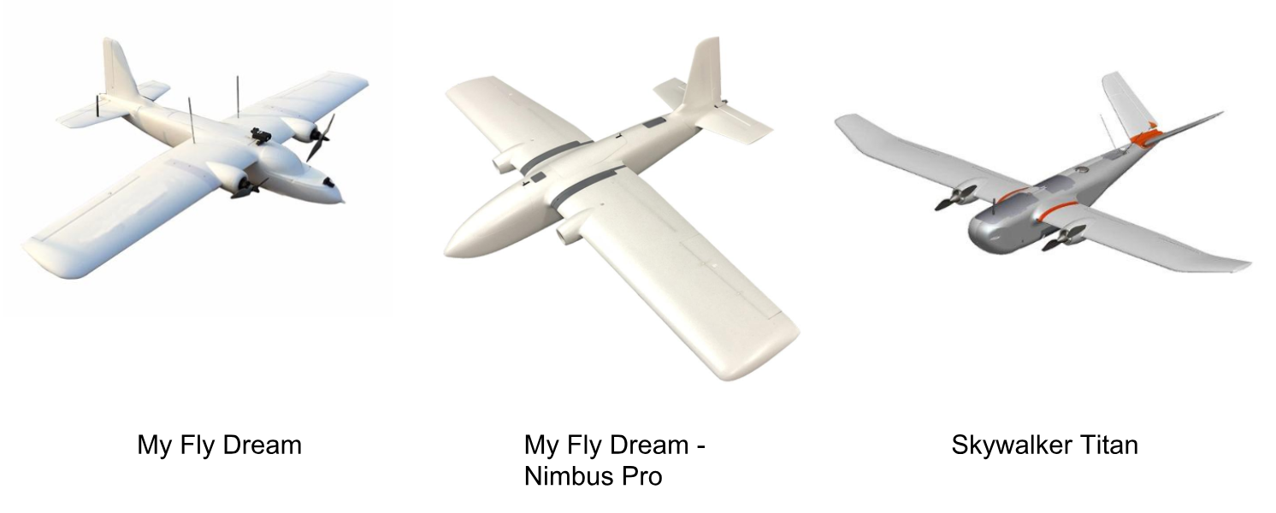
\includegraphics[scale=0.5]{Planes1}
	\caption{Three commercially available airframes investigated. According to Dr. McLain, Skywalker Titan is incredibly unstable. Images taken from banggood.com.}
	\label{planes1}	
\end{figure}

\section{Conclusion}

The Modified Nimbus Pro was selected as it scored highest on the selection matrix. Although it will require slightly more time to build, we believe that the increase in performance justifies the time expense. The concept and how it responds to our Key Success Measures are described in greater detail in the Airframe Concept Description.

\end{document}